\documentclass[landscape]{article}
\usepackage[a4paper,margin=3mm,landscape]{geometry}
\usepackage[scaled=0.92]{helvet}
\usepackage{multicol, multirow}
\usepackage{makecell}
\usepackage{array} 
\usepackage[table]{xcolor}
\usepackage{enumitem} 
\usepackage{amssymb}
\usepackage{graphicx}
\setlist{nosep}

\graphicspath{{./images/}}

\pdfinfo{
    /Title (CS2106 Cheatsheet.pdf)
    /Creator (TeX)
    /Producer (pdfTeX 1.40.0)
    /Author (Selwyn Ang)
    /Subject (CS2106)
    /Keywords (CS2106, Cheatsheet, NUS, Introduction to Operating Systems) 
}

% Turn off header and footer
\pagestyle{empty}


\makeatletter
\DeclareRobustCommand\smaller{\@setfontsize\smaller{6pt}{6.5pt}}
\makeatother

% redefine section commands to use less space
\makeatletter
\renewcommand{\section}{\@startsection{section}{1}{0mm}%
  {-0.1ex plus -0.1ex minus -0.1ex}%
  {0.1ex plus .1ex minus 0.1ex}%
{\normalfont\small\bfseries}}
\renewcommand{\subsection}{\@startsection{subsection}{2}{0mm}%
  {-0.1ex plus -0.1ex minus -0.1ex}%
  {0.1ex plus .1ex minus 0.1ex}%
{\normalfont\scriptsize\bfseries}}
\renewcommand{\subsubsection}{\@startsection{subsubsection}{3}{0mm}%
  {-0.1ex plus -0.1ex minus -0.1ex}%
  {0.1ex plus .1ex minus 0.1ex}%
{\normalfont\smaller\bfseries}}%
\makeatother



\renewcommand{\familydefault}{\sfdefault}
\renewcommand\rmdefault{\sfdefault}
%  makes nested numbering (e.g. 1.1.1, 1.1.2, etc)
\renewcommand{\labelenumii}{\theenumii}
\renewcommand{\theenumii}{\theenumi.\arabic{enumii}.}
\renewcommand\labelitemii{•}
\renewcommand\labelitemiii{•}

\setlength{\parindent}{0pt}
\setlength{\parskip}{0pt plus 0.5ex}
\setlength{\columnsep}{0.2cm}
%% adjust spacing for all itemize/enumerate
\setlength{\leftmargini}{0.5cm}
\setlength{\leftmarginii}{0.5cm}
\setlist[itemize,1]{leftmargin=2mm,labelindent=1mm,labelsep=1mm}
\setlist[itemize,2]{leftmargin=2mm,labelindent=1mm,labelsep=1mm}
\setlist[itemize,3]{leftmargin=2mm,labelindent=1mm,labelsep=1mm}
\setlist[enumerate,1]{leftmargin=2mm,labelindent=1mm,labelsep=1mm}
\setlist[enumerate,2]{leftmargin=2mm,labelindent=1mm,labelsep=1mm}
\setlist[enumerate,3]{leftmargin=2mm,labelindent=1mm,labelsep=1mm}

% tightcenter
\newenvironment{tightcenter}{%
  \setlength\topsep{0pt}
  \setlength\parskip{0pt}
  \begin{center}
    }{%
  \end{center}
}

% boxed
\newenvironment{tightbox}{%
  \setlength\topsep{0pt}
  \setlength\parskip{0pt}
  \begin{center}
    \begin{tabular}{|@{\hspace{\dimexpr\fboxsep+0.5\arrayrulewidth}}c@{\hspace{\dimexpr\fboxsep+0.5\arrayrulewidth}}|}
      \hline
    }
    {%
    \\ \hline
    \end{tabular}
  \end{center}
}

% fixed width box
\newenvironment{fixedbox}[1][0.7]{
  \setlength\topsep{0pt}
  \setlength\parskip{0pt}
  \begin{center}
    \begin{tabular}{|>{\centering\arraybackslash}m{#1\linewidth}|}
    \hline
  }{
  \\ \hline
  \end{tabular}
  \end{center}
}

% definition of a new term
\usepackage{soul}
\definecolor{paleyellow}{RGB}{251,243,218}
\newcommand{\definition}[2][]{\sethlcolor{paleyellow}\hl{\textbf{#2}} #1  $\rightarrow$}
% inline definition
\newcommand{\ildefinition}[1]{\sethlcolor{paleyellow}\hl{\textbf{#1}}}

% important note (attention)
\newcommand{\attention}{{\color{red}\textbf{! }}}

% nice proof
\newenvironment{niceproof}[1][Proof]
{%
  \sbox0{\textit{#1}. }%
  \list{}{\labelwidth\wd0 \leftmargin\wd0 \labelsep 0pt }
\item[\usebox0]}
  {\endlist}


\usepackage{color, soul}
\usepackage{listings}
\usepackage{inconsolata}

\definecolor{codegreen}{rgb}{0,0.6,0}
\definecolor{codegray}{rgb}{0.5,0.5,0.5}
\definecolor{codepurple}{HTML}{C42043}
\definecolor{backcolour}{HTML}{F2F2F2}
\definecolor{bookColor}{cmyk}{0,0,0,0.90}

\newcommand{\code}[1]{\texttt{\sethlcolor{backcolour}\hl{$\,$#1$\,$}}}

% SQL code blocks
% define SQL styles
\lstdefinestyle{mySQL}{%
  language=SQL,
  backgroundcolor=\color{backcolour},
  commentstyle=\color{codegreen},
  keywordstyle=\color{codepurple},
  numberstyle=\numberstyle,
  stringstyle=\color{codepurple},
  basicstyle=\scriptsize\ttfamily,
  breaklines=true,
}



% --------------------------------------------------------

\begin{document}
\raggedright
\tiny
\begin{multicols*}{5}
    \setlength{\columnseprule}{0.25pt}

    \begin{tightcenter}
        \fbox{%
          \parbox{0.8\linewidth}{\centering \textcolor{black}{
              {\Large\textbf{CS2106}}
            \\ \normalsize{AY23/24 SEM 2}}
            \\ {\footnotesize \textcolor{gray}{github/SelwynAng}}
          }%
        }
    \end{tightcenter}
    
    \section{Introduction to OS}
    \subsection{OS Basic Concepts}
    \begin{itemize}
      \item \textbf{Definition of OS:} Program that acts as intermediary btw. computer user \& computer hardware
      \item \textbf{Types of OS:}
      \begin{enumerate}
        \item \underline{Mainframe OS}: Executes user program one at a time (but simple batch processing is inefficient since CPU idle when performing I/O)
        \item \underline{Time-sharing OS}: Allows multiple users to interact with machine, user job scheduling (Illusion of concurrency); Provides sharing of CPU time, memory, storage; Virtualisation of hardware 
      \end{enumerate}
      \item \textbf{Motivations of OS:}
      \begin{enumerate}
        \item \underline{Abstraction:} Hides low level details, present common high level functionality to user; Provides efficiency \& portability, but latency is present
        \item \underline{Resource Allocator:} Multiple programs can execute simultaneously $\rightarrow$ OS manages all resources $\rightarrow$ Arbitrate conflicting requests
        \item \underline{Control Program:} OS controls execution of programs $\rightarrow$ Prevents errors \& improper use of computer, provides security \& protection
      \end{enumerate}
    \end{itemize}

    \subsection{OS Structures}
    \begin{itemize}
      \item \textbf{Generic OS}: OS is known as Kernel (Deals with hardware, provides system call interface, special code for interrupt handlers, device drivers)
      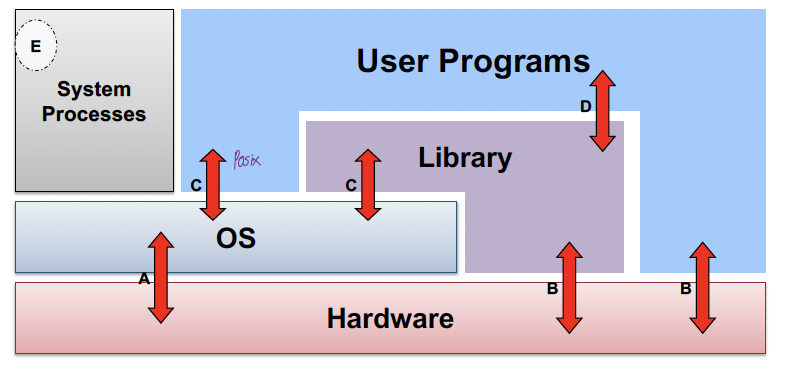
\includegraphics[width=0.9\linewidth]{01_general_os.png}
      \item \textbf{Monolithic OS}: Kernel == 1 big program, (+) good performance (-) highly coupled components, complicated internal structure, eg. Most Unix variants, Windows
      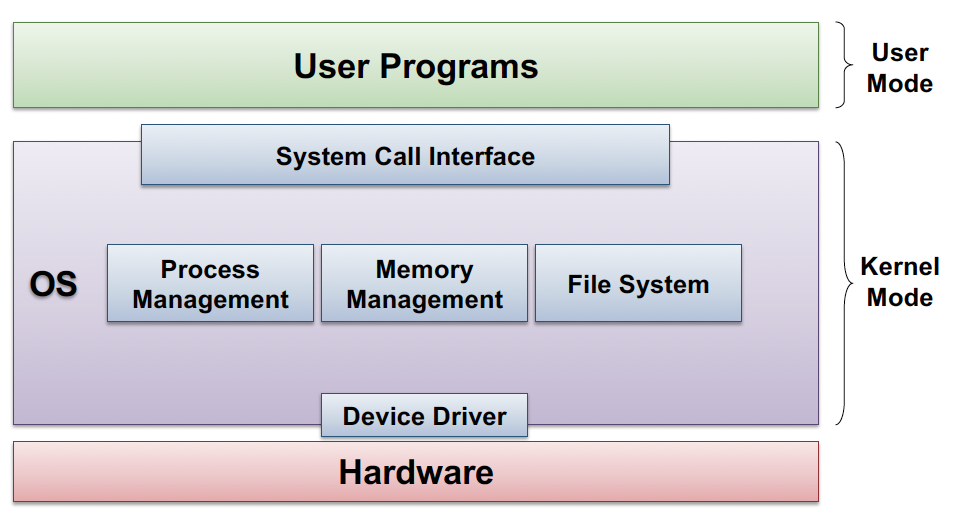
\includegraphics[width=0.9\linewidth]{02_monolithic_os.png}
      \item \textbf{Microkernel OS}: Kernel is small, provides basic \& essential facilities, uses IPC to communicate, (+) More modular, robust, better isolation, protection between kernel \& user spaces (-) lower performance
      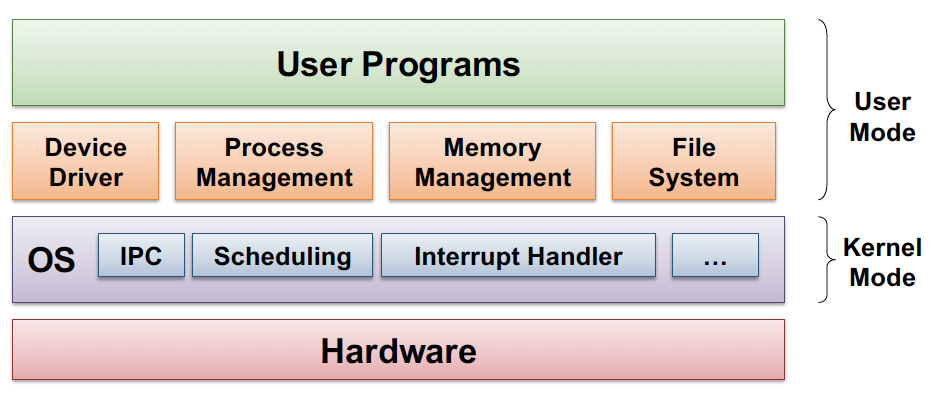
\includegraphics[width=0.9\linewidth]{03_microkernel_os.png}
      \item \textbf{Layered Systems OS:} Generalisation of Monolithic system, hierarchy of layers where upper layers make use of lower layers $\rightarrow$ Lowest layer is hardware, Highest layer is user interface
      \item \textbf{Client-Server Model:} Variation of Microkernel where server process is built on top of microkernel, client \& server process can be on separate machine
    \end{itemize}

    \subsection{Virtual Machines}
    \begin{itemize}
      \item \textbf{Definition:} Software emulation of hardware, normal OS then run on top of VM (aka. Hypervisor)
      \item \textbf{Type 1 Hypervisor:} Runs directly on hardware (more efficient), provides individual VMs to guest OSes
      \item \textbf{Type 2 Hypervisor:} Runs on host OS (more overhead), guest OS runs inside VM (more common for normal users)
    \end{itemize}


\end{multicols*}
\end{document}
